\chapter{Análisis experimental}
Este capítulo presenta la evaluación experimental del AE multiobjetivo propuesto para resolver el problema de sincronización de semáforos en el Corredor Garzón. Se describen las instancias del problema y la plataforma de ejecución utilizada en la evaluación experimental. A continuación se estudia la configuración paramétrica del AE con el objetivo de obtener una mejor calidad de resultados, se describen los experimentos de validación y se reportan los resultados numéricos. Finalmente se ofrece un breve análisis de la eficiencia computacional del AE propuesto.

\section{Plataforma de ejecución y desarrollo}

Dada la complejidad del problema, el análisis experimental se realizó en la plataforma de cómputo de alto desempeño Cluster FING, de la Universidad de la República~\citep{nesmachnow2010computacion}. Para acelerar el tiempo de procesamiento se ejecuta el AE en paralelo, distribuyendo la carga de procesar las simulaciones de tráfico en múltiples núcleos de cómputo. El Cluster FING cuenta con procesadores AMD Opteron 6272 de 2.09GHz, con 64 núcleos, 48GB RAM, y sistema operativo CentOS Linux 6.5.

%Las pruebas incluidas en el análisis experimental utilizaron entre 4 y 32 núcleos de procesamiento. Dada la naturaleza de recursos compartidos del Cluster, no siempre es posible contar con la misma cantidad de recursos disponibles, además, para la mayoría de las pruebas el número de núcleos no es relevante. El numero de núcleos utilizados será tenido en cuenta, cuando se realice el análisis de eficiencia computacional detallado al final de este capítulo.


\section{Experimentos de calibración paramétrica del AE}
Se llevó a cabo un análisis previo para determinar el mejor valor de los parámetros del AE propuesto. Este análisis tiene como objetivo obtener una mejor calidad de resultados. El análisis consistió en determinar valores adecuados para el \emph{tiempo de simulación} de los escenarios planteados en SUMO, el \emph{criterio de parada} y el \emph{tamaño de la población} del AE. Posteriormente, se realizó un ajuste de las \emph{probabilidades de cruzamiento} y de \emph{mutación} en el AE. 

%Los parámetros que se ajustan incluyen el \emph{tiempo de simulación} que se refiere al parámetro del simulador SUMO para determinar la duración de la simulación. También se configura el \emph{criterio de parada} que indica el método usado para detener el algoritmo y el \emph{tamaño de la población} que representa la cantidad de individuos de la población utilizada en el AE. Finalmente se ajustan los parámetros de \emph{probabilidad de mutación y probabilidad de cruzamiento}. Estos parámetros serán descritos en detalle en las siguientes secciones.

Los experimentos de ajuste paramétrico se realizaron sobre tres escenarios de tráfico: \emph{i}) \emph{tráfico bajo}, con 30 ómnibus y 500 vehículos; \emph{ii}) \emph{tráfico medio}, con 60 ómnibus y 1000 vehículos; y \emph{iii}) \emph{tráfico alto}, con 120 ómnibus y 2000 vehículos. Estos escenarios no incluyen datos recabados de la realidad (como el tráfico vehicular o la frecuencia de los ómnibus), para no ajustar los parámetros a un caso particular.

En el ajuste paramétrico los primeros parámetros que se definen son: el tiempo de simulación, el criterio de parada y el tamaño de población. Luego de establecidos los valores para los parámetros mencionados, se realizan las pruebas para todas las combinaciones de probabilidad de cruzamiento y mutación buscando los valores con los cuales el AE obtiene una mejor calidad de resultados.

%La plataforma Cluster FING donde se desarrolla el análisis experimental permite disponer tanto de la métrica del tiempo real que dura la ejecución, así como también el tiempo secuencial, es decir la suma del tiempo de procesamiento de todos los procesadores involucrados en la evaluación del algoritmo. Cuando se realizan comparaciones en los tiempos de ejecución se utiliza el tiempo secuencial que es independiente de la cantidad de procesadores utilizados en las pruebas. 

%\subsection{Pesos de la función de fitness}

%Para el análisis experimental la función de \emph{fitness} del algoritmo (\ref{eq:funcion_fitness}) tendrá los pesos \emph{$w_1$ = $w_2$ = 1}. Estos valores dan pesos equitativos tanto a ómnibus como a otros vehículos, por lo que no existe prioridad para uno u otro. Más adelante se realizarán experimentos con otras variantes.


\subsection{Tiempo de simulación}
El tiempo de simulación refiere a la duración de la ejecución de una simulación usando SUMO. Es un parámetro que se puede configurar y permite tener un mejor control sobre los tiempos totales de ejecución del algoritmo.

Se establece un tiempo de simulación de 4000 \emph{steps} (medida interna de tiempo del simulador) que representa 66 minutos en la realidad. El tiempo de ejecución real de cada simulación depende de la plataforma computacional utilizada y de la cantidad de vehículos considerados en el escenario, variando entre los 5 y 20 segundos. Para cada escenario, se valida que más del 80\% de los vehículos completen la simulación (lleguen a sus destinos). 
%Se realizaron 10 ejecuciones del AE para cada uno de los tres tipos de tráfico, comprobando que se cumplía el criterio anterior.


\subsection{Criterio de parada}
Se decidió utilizar como criterio de parada un determinado número de generaciones. Este criterio permite estandarizar las pruebas y evaluar una comparación justa entre los distintos escenarios de tráfico. Para determinar el 
criterio de parada del AE se busca un compromiso entre los resultados numéricos y el tiempo de ejecución. 
Se realizaron 10 ejecuciones del AE para cada tipo de tráfico, y los resultados indicaron que el mejor valor de \emph{fitness} no varía significativamente luego de la generación 400, por lo que se decidió utilizar un criterio de parada de 500 generaciones, que involucra un tiempo de ejecución del AE en un margen razonable (entre 1 y 24 horas). 

%En la Figura \ref{fig:criterio_parada} se aprecia como el valor del mejor \emph{fitness} no presenta grandes variaciones luego de la generación 400, además el tiempo de ejecución real se encuentra dentro del margen pautado. La gráfica no muestra todos los valores obtenidos en los experimentos de configuración, sólo algunos valores representativos para una mejor visualización.

%\begin{figure}[ht]
%\centering
%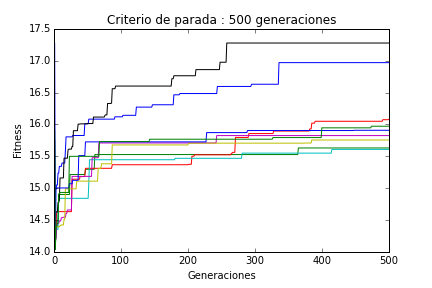
\includegraphics[width=0.8\linewidth]{Figures/criterio_parada}
%\caption[Gráfica de la evolución de los valores de fitness. ]{Gráfica de la evolución de los mejores valores de fitness para %establecer el criterio de parada.}
%\label{fig:criterio_parada}
%\end{figure}

\subsection{Tamaño de la población}

Para determinar el número de individuos de la población se tiene en cuenta el valor de \emph{fitness} obtenido por el AE, su tiempo de ejecución y los recursos computacionales. Teniendo en cuenta la distribución de recursos computacionales para realizar las simulaciones de tráfico, el número máximo de individuos (64) queda determinado por la cantidad de núcleos en un nodo del Cluster FING. Además, se estudian poblaciones de 32 y 48 individuos.
%Teniendo en cuenta que la mejor distribución para realizar las simulaciones es de un individuo por núcleo, se determina que la máxima cantidad de individuos en la población será de 64. Luego se establecen dos valores más para completar el análisis, con un tamaño de población de 32 y 48 individuos. Se eligen estos valores ya que no son lo suficientemente bajos y se logra una distribución adecuada de individuos en la infraestructura.

La Tabla \ref{table:parametro_poblacion} reporta los resultados de 10 ejecuciones del AE por cada tipo de tráfico estudiado, con diferente número de individuos en la población. Los resultados indican que no existen diferencias significativas en los valores de fitness, por lo cual se elige un tamaño de población de 32 individuos, teniendo en cuenta el menor tiempo de ejecución del AE y el menor uso de recursos computacionales.

\begin{table}[!ht]
	\renewcommand{\arraystretch}{1.0}
\renewcommand{\tabcolsep}{8pt}
	\caption{Resultados del análisis de diferentes valores para el tamaño de población.}
	\label{table:parametro_poblacion}
	\centering
	\begin{tabular}{rrrrrp{2cm}}
		\toprule
		\multirow{2}{*}{\textit{\#población}}& &
		\multicolumn{2}{c}{\textit{fitness}} & \multirow{2}{*}{\textit{tiempo de ejecución (m)}} \\
		\cline{3-4} \\[-9pt]
		& & \textit{mejor}
		& \textit{promedio$\pm \sigma$}
		\\
		\midrule
		32 & & {17.28} & 16.37$\pm$0.5 & 10184$\pm$526\\
		48 & & {16.19} & 15.84$\pm$0.3 & 6772$\pm$256\\
		64 & & {17.27} & 16.46$\pm$0.6 & 4853$\pm$155\\
		\bottomrule
	\end{tabular}
\end{table}

\subsection{Probabilidades de cruzamiento y mutación}
Para el análisis paramétrico de la probabilidad de cruzamiento ($p_C$) se consideraron tres valores candidatos: \{0.5, 0.8, 1\} y para la probabilidad de mutación ($p_M$) los valores \{0.01,  0.05,  0.1\}. De las nueve combinaciones posibles, se realizaron tres ejecuciones independientes del AE para cada uno de los tres tipos de tráfico (bajo, medio y alto).  

\begin{figure}[H]
\begin{minipage}[t]{0.4\linewidth}
\begin{table}[H]
	\renewcommand{\arraystretch}{1.0}
\renewcommand{\tabcolsep}{4pt}
	\centering
	\begin{tabular}{rrr}
		\toprule
		$p_C$&
		$p_M$ &
		\textit{fitness prom.$\pm \sigma$}\\
		\midrule
		0.5 & 0.01  &  16.09$\pm$0.30\\
		0.5 & 0.05 &  15.60$\pm$0.17\\
		0.5 & 0.1  &  16.16$\pm$0.42\\
		0.8 & 0.01  &  16.04$\pm$0.55\\
		0.8 & 0.05  &  15.85$\pm$0.32\\
		0.8 & 0.1  &  16.08$\pm$0.34\\
		1 & 0.01 &  16.08$\pm$0.45\\
		1 & 0.05 &  15.82$\pm$0.34\\
		1 & 0.1 &  16.04$\pm$0.25\\
		\bottomrule
\\[-9pt]
	\end{tabular}
\end{table}
\end{minipage}
\begin{minipage}[t]{0.6\linewidth}
\begin{figure}[H]
	\centering
	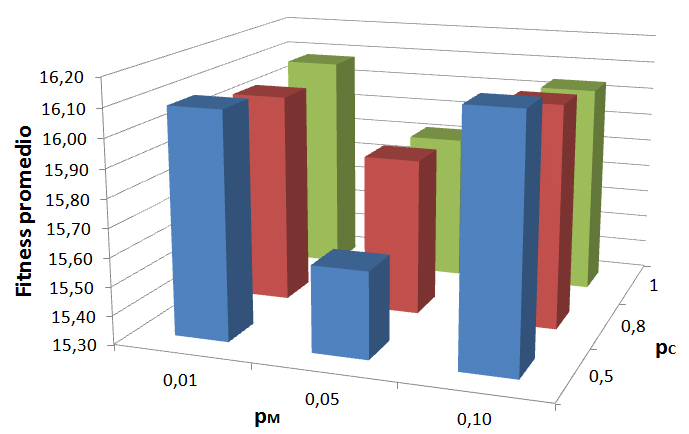
\includegraphics[width=1.0\linewidth]{Figures/grafica_mutacion_cruzamiento}
	\label{fig:grafica_mutacion_cruzamiento}
\end{figure}
\end{minipage}
	\caption{Resultados 
%(\textit{fitness}) 
del análisis de la probabilidad de cruzamiento ($p_C$) y mutación ($p_M$)}
	\label{table:parametro_mutacion_cruzamiento}
\end{figure}
 
El análisis estadístico muestra que los resultados siguen una distribución normal, siendo posible aplicar el test de Student para estudiar las distribuciones. Al comparar los resultados de las combinaciones que obtienen el mejor (0.5--0.1) y el peor (0.5--0.05) promedio de fitness, el test de Student reporta un valor $t(x)= 0.07$, que permite rechazar la hipótesis nula con un nivel de significancia de 0.1, indicando que existe evidencia estadística para elegir la combinación con el mejor promedio.

Entre las dos mejores combinaciones (0.5--0.1) y (0.5--0.01) no existe una diferencia significativa, siendo posible utilizar cualquiera de ambas. En la evaluación experimental se utiliza la combinación de parámetros (0.5-0.01) por su buen promedio y baja desviación estándar.


\section{Descripción de escenarios}
Esta sección presenta los escenarios que serán evaluados experimentalmente. El primero es el escenario base que representa la realidad actual y el segundo es un escenario alternativo que presenta modificaciones respecto al caso base, con el objetivo de mejorar las velocidades promedio de los vehículos.

\subsection{Caso base o realidad actual del corredor}
El caso base representa la situación actual en términos de tráfico, red vial y sincronización de semáforos del corredor Garzón. Se simulan las instancias realistas desarrolladas en el capítulo 4 para obtener las velocidades promedio de ómnibus y otros vehículos y poder comparar con los resultados numéricos luego de aplicar el AE propuesto.  

Sobre el mapa base se generan tres escenarios de tráfico: 1) \textit{tráfico medio}, que representa los datos obtenidos en el trabajo de campo (2000 vehículos y 70 ómnibus); 2) \textit{tráfico bajo}, que se construye reduciendo en un 50\% la cantidad de vehículos y el tiempo de espera en las paradas de ómnibus, ya que existirán menos personas utilizando el transporte público (1000 vehículos y 70 ómnibus); y 3)  \textit{tráfico alto}, en el que se aumenta 50\%  la cantidad de vehículos y el tiempo de espera en la parada de los ómnibus (3000 vehículos y 70 ómnibus). Las frecuencias de ómnibus se mantienen, ya que en la realidad no son alteradas cuando cambia la densidad de tráfico. El valor de 50\% para el aumento y reducción del número de vehículos se infirió al analizar datos de la zona de Garzón de años anteriores, proporcionados por la IMM.
 

\subsection{Escenario alternativo}

Para mostrar la utilidad que tienen las simulaciones de tráfico, se genera un escenario alternativo basado en el escenario base al que se le modifican los aspectos que se consideran influyen negativamente en la circulación del tráfico. Una de las ventajas principales de las simulaciones de tráfico es que no requiere gran inversión monetaria ni de tiempo y que no modifica la infraestructura del lugar, por lo que se pueden generar distintas pruebas para encontrar aquellas que logren el objetivo buscado, por ej. la mejora en la circulación del tráfico.

Analizando los puntos que se entienden podrían atentar contra el buen funcionamiento del corredor, se realizan algunas modificaciones al escenario base para intentar mejorarlo. 
%El objetivo no es encontrar la mejor alternativa, sino dar una de las muchas alternativas que se pueden generar y probar con las simulaciones de tráfico.
 % Ya que pueden existir limitaciones o reglas que no estamos tomando en cuenta y que deben cumplirse en la realidad.

Entre los cambios propuestos para el escenario alternativo se encuentran: eliminación de paradas y pasajes peatonales, alternancia de paradas y modificación de reglas de los semáforos.

\subsection{Detalles del escenario alternativo}
Los cambios propuestos para el escenario alternativo incluyen la eliminación de paradas, semáforos y pasajes peatonales y la posibilidad de alternar paradas. Se estudiaron otras propuestas como por ejemplo construir calles paralelas a Garzón o incorporar nuevas reglas de tráfico en los cruces (por ej. permitir doblar a la derecha con roja) como existen en otros países pero fueron descartadas por la poca viabilidad real de implementarlas.

\subsubsection{Eliminación de paradas}
Se consideraron eliminar paradas que cumplieran con las siguientes características: que no estuvieran próximas a una calle principal y que existiera otra parada cercana para no afectar a los pasajeros realizando un traslado excesivo.  Se seleccionaron solamente dos paradas para que su eliminación no tuviera un impacto negativo en el funcionamiento diario del Corredor y que cumplieran los criterios mencionados anteriormente. Las paradas elegidas están ubicadas en las intersecciones de Garzón con las calles Ariel y Casavalle.

\subsubsection{Eliminación de pasajes peatonales}
En la actualidad, existen en el corredor Garzón tres pasajes peatonales con semáforos que detienen el tráfico. El objetivo buscado al proponer su eliminación es aumentar la velocidad promedio de los vehículos circulantes. Dos de los pasajes peatonales controlan el flujo peatonal de las esquinas en la Plaza Vidiella y Camino Besnes e Irigoyen (sin pulsador en funcionamiento). En el escenario alternativo estos dos pasajes fueron cambiados por una señalización de {PARE} en la calle transversal al corredor Garzón. El tercer pasaje es netamente peatonal y se encuentra ubicado frente a la Facultad de Agronomía, entre las calles Millán y Orticochea, el cual fue eliminado en el escenario alternativo. Una opción para no eliminar físicamente los pasajes peatonales y mantener los resultados obtenidos, es implementar el pasaje peatonal mediante puentes por encima del corredor Garzón.

\subsubsection{Alternar paradas}

Uno de los problemas del ómnibus es su baja aceleración, por lo que cada vez que se detiene en un semáforo o en una parada, demora en retornar a una velocidad aceptable. Al reducir la cantidad de paradas donde un ómnibus tiene que detenerse se mejora la velocidad promedio.
La línea G recorre el corredor Garzón de punta a punta y es cubierta por las empresas COETC y CUTCSA. Una posibilidad para alternar paradas consiste en dividir las paradas por empresa y compartir las ganancias generadas equitativamente u otro método para equiparar el pasaje transportado. 

La Figura \ref{fig:paradas_alternadas} brinda un ejemplo donde una empresa se detendrá en las paradas pares, la otra en las impares y algunas paradas con más cantidad de pasajeros serán realizadas por las dos. Cada empresa viajará por el corredor con una frecuencia de 4 minutos (como en la actualidad). Si se reduce el número de paradas donde se detiene un ómnibus, aumentará su velocidad promedio y no se deberá resentir en demasía el servicio, ya que la disminución de la frecuencia en una parada se contrarresta con el aumento promedio de velocidad.

%El cambio de alternar paradas es el que más aumenta la velocidad media y tal vez es uno de los más sencillos de implementar en la realidad.


\begin{figure}[ht]
	\centering
	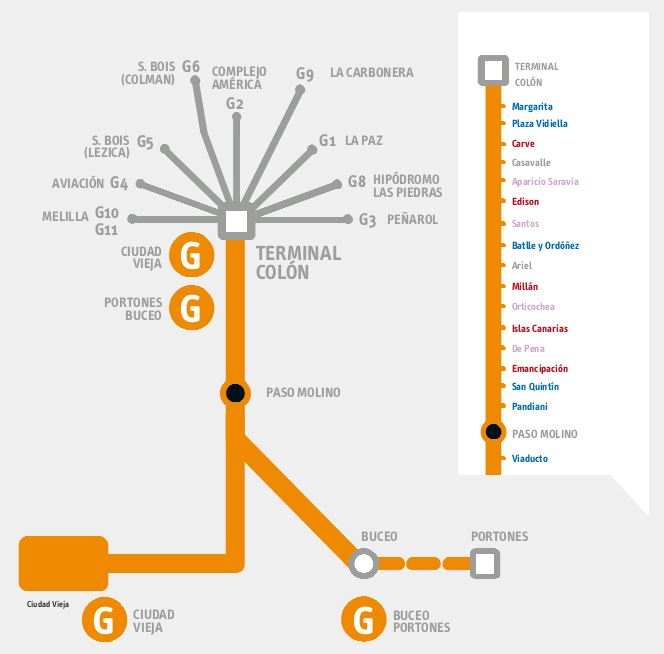
\includegraphics[width=0.9\linewidth]{Figures/paradas_alternativas}
	\caption[Gráfico de las paradas alternativas.]{Gráfico de las paradas alternativas. Gris: Parada Eliminada. Azul: línea G de COETC y de CUTCSA. Rojo: línea G de COETC. Violeta: G de CUTCSA. - Imagen original extraída de montevideo.gub.uy}
	\label{fig:paradas_alternadas}
\end{figure}



\subsubsection{Cambio básico de semáforos}
Al hacer el relevamiento de los datos obtenidos de la configuración de los semáforos del Corredor Garzón, se constató que en todas las intersecciones en donde una línea de ómnibus que circula por el corredor tiene un viraje a la izquierda, se hace detener el tránsito de la derecha de la misma, cada vez que el corredor central tiene la luz verde. Esto no parece tener mucho sentido, ya que los vehículos podrían seguir circulando por el corredor sin ningún tipo de problema. El carril que hay que detener cuando una línea dobla a la izquierda es el de la izquierda del ómnibus, pero no los dos carriles al mismo tiempo. No se tiene conocimiento si esta decisión corresponde a un error en la configuración, un tema de costos o facilidad para manejar los dos semáforos de los carriles paralelos juntos. Como esto ocurre en varias intersecciones y en ambos sentidos, el cambio mejora la velocidad promedio de los autos que circulan por los dos carriles.

Este cambio se aplicó en las siguientes intersecciones: \emph{i}) \emph{Islas Canarias}, dobla línea 409 hacia la izquierda, orientado a Colón (Norte); \emph{ii}) \emph{Camino Ariel}, doblan líneas como la  2 y la 148 hacia la izquierda, orientado a Paso Molino (Sur); y \emph{iii}) \emph{Camino Casavalle}, dobla línea 174 hacia la izquierda, orientado a Paso Molino (Sur).

%\begin{itemize}
  % \item Islas Canarias: dobla línea 409 hacia la izquierda, orientado a Colón (Norte).
	%\item Camino Ariel: doblan líneas como la  2 y la 148 hacia la izquierda, orientado a Paso Molino (Sur). 
	%\item Camino Casavalle: dobla línea 174 hacia la izquierda, orientado a Paso Molino (Sur). 
%\end{itemize}

\section{Resultados}
Esta sección muestra los resultados obtenidos en la simulación del caso base, y los resultados numéricos del AE. El objetivo es comparar la velocidad promedio de ómnibus y vehículos con la realidad actual 

%. Se presenta la simulación del escenario alternativo y la posterior evaluación. %Además se realizan estudios sobre cambios en la función de \emph{fitness} del AE y un breve análisis de la eficiencia computacional.


\subsection{Resultados de la simulación del caso base.}

Los resultados de las simulaciones para los diferentes tráficos en la realidad actual, tomada como caso base para comparar los resultados del AE propuesto, se reportan en la Tabla \ref{table:resultado_caso_base}. Los resultados representan la realidad actual del Corredor Garzón: la velocidad promedio en tráfico medio es de 14.59 km/h para los ómnibus y de 28.81 km/h para los vehículos. Estos valores se corresponden con los que surgen del análisis de datos reales (trazas de GPS de ómnibus) proporcionados por la IMM(14.5 km/h), verificando que el modelo propuesto se aproxima significativamente a la realidad.

%En la tabla \ref{table:resultado_caso_base} se pueden ver los resultados obtenidas para las diferentes instancias de tráfico simulado para el caso base. Estos datos representan la realidad actual del Corredor Garzón. Como se aprecia, la velocidad promedio de los ómnibus en tráfico medio es de 14.59 km/h, siendo 14.5 km/h el valor que se obtuvo de analizar los datos reales proporcionados por la IMM, lo que verifica que el modelo se aproxima significativamente a la realidad. En la tabla  \ref{table:resultado_caso_base} el valor de \emph{fitness} se corresponde con la evaluación de la función de \emph{fitness} (Ecuación \ref{eq:funcion_fitness_generica}) utilizando las velocidades de ómnibus y otros vehículos obtenidas para cada tipo de tráfico.
 
\begin{table}[H]
	\renewcommand{\arraystretch}{1.0}
\renewcommand{\tabcolsep}{12pt}
	\caption[Resultados numéricos del caso base.]{Resultados numéricos del caso base: velocidad promedio para ómnibus (\textit{vpb}) y vehículos (\textit{vpv}) para los distintos tipos de tráfico.}
	\label{table:resultado_caso_base}
	\centering
	\begin{tabular}{lrrr}
		\toprule
		\textit{escenario}  &
		\textit{vpb}(km/h) &
		\textit{vpv}(km/h) &
		\textit{fitness} \\
		\midrule
		tráfico bajo & 15.89  & 32.45& 13.42\\
		tráfico medio & 14.59  & 28.81& 12.05\\
		tráfico alto & 14.31  & 26.36& 11.30\\
		\bottomrule
	\end{tabular}
\end{table}
 
 %En el caso base no se calcula la desviación standard ya que los valores obtenidos son deterministas (velocidad promedio de ómnibus, de otros vehículos y el valor de \emph{fintess}), pues siempre se simulan los mismos recorridos de los vehículos y la misma configuración de los semáforos. Cuando se aplica el AE, se generan nuevas configuraciones de semáforos, por lo que se obtiene un valor diferente de la velocidad promedio y del valor de \emph{fitness}, calculándose la desviación standard para evaluar la robustez de los resultados.


\subsection{Resultados numéricos de la evaluación }

Los resultados de aplicar la optimización de las velocidades de ómnibus y otros vehículos con el AE propuesto se reportan en la Tabla \ref{table:resultado_caso_algoritmo}. Se presentan los valores promedio de las velocidades para ómnibus y otros vehículos, el valor de \emph{fitness} resultante y la mejora porcentual del valor de \emph{fitness} obtenida en comparación con el valor obtenido en el caso base.

Se realizaron 20 ejecuciones independientes del AE para cada tipo de tráfico. Al aplicar el AE se generan nuevas configuraciones de semáforos, por lo que se obtiene un valor diferente de la velocidad promedio y del valor de \emph{fitness}, calculándose la desviación estándar ($\sigma$) para evaluar la robustez de los resultados.

%Como se aprecia en la tabla \ref{table:resultado_caso_algoritmo}, el AE mejora la velocidad promedio tanto de ómnibus como de otros vehículos en los tres tipos de tráfico estudiados. Además, la velocidad media de los vehículos se mantiene en un rango mucho más ajustado que en el caso original al variar el tráfico. Las mejoras logradas en el \emph{fitness} son de hasta 24\% con respecto al caso base. A continuación se describe el análisis estadístico para comprobar la mejora.


\begin{table}[H]
	\renewcommand{\arraystretch}{1.05}
\renewcommand{\tabcolsep}{4pt}
	\caption[Resultados numéricos del caso base.]{Resultados numéricos del AE: velocidad promedio para ómnibus (\textit{vpb}) y vehículos (\textit{vpv}) para los distintos tipos de tráfico.}
	\label{table:resultado_caso_algoritmo}
	\begin{tabular}{lrrrrrrr}
		\toprule
		\multirow{2}{*}{\textit{instancia}}&
		\multirow{2}{*}{\textit{vbp}(km/h)}&
		\multirow{2}{*}{\textit{vpv}(km/h)}&
		\multicolumn{2}{c}{\emph{fitness}}&  &
		\multicolumn{2}{c}{mejora \emph{fitness} (\%)}\\  
		\cline{4-5} \cline{7-8}\\[-9pt]
		&     &     & \multicolumn{1}{c}{promedio$\pm\sigma$} & \multicolumn{1}{c}{mejor} &  & \multicolumn{1}{c}{promedio} & \multicolumn{1}{c}{mejor} \\ 
		\midrule
		\textit{tráfico bajo} & 17.92$\pm$0.18 & 34.30$\pm$0.40 & 14.50$\pm$0.14 & 14.88 & & 8.04 & 10.8  \\
		\textit{tráfico medio} & 16.95$\pm$0.32 & 33.29$\pm$0.29 & 13.95$\pm$0.15 & 14.19 & & 15.7& 17.7\\
		\textit{tráfico alto} & 16.51$\pm$0.61  & 32.90$\pm$0.25& 13.72$\pm$0.17 & 14.04 & & 21.4& 24.2\\    
		\bottomrule        
	\end{tabular}
\end{table}


Los resultados reportados en la Tabla \ref{table:resultado_caso_algoritmo} indican que la optimización utilizando AE permite mejorar la velocidad promedio de los ómnibus y de otros vehículos en los tres tipos de tráfico estudiados. Además, las soluciones cuentan con mayor robustez, ya que al variar el tráfico la velocidad media de los vehículos se mantiene en un rango mucho más ajustado que en el caso original. Las mejoras logradas por el AE con respecto al caso base son de hasta \textbf{24\%} en el \emph{fitness} y las mejoras en las velocidades son de hasta \textbf{15.3\%} en la velocidad promedio de ómnibus y \textbf{24.8\%} en la velocidad promedio de otros vehículos, al comparar con la realidad actual.

El análisis estadístico 
%para validar los porcentajes de mejora 
indicó que los resultados 
%obtenidos 
siguen una distribución normal. Por lo tanto se puede aplicar el criterio de \textit{significancia estadística de comparación de medias} para validar los resultados:
%, que indica que 
un método $A$ (en este caso, la optimización con AE) es mejor que otro método $B$ (en este caso, el escenario base) si los resultados de $A$ y B cumplen que 
%\begin{equation}
%\label{eq:funcion_significancia}
$
\left |f_{avg}(A) - f_{avg}(B)  \right | > \max(\sigma(f_A),\sigma(f_B))
$.
%\end{equation}
%
%En el caso estudiado, A representa la optimización de tráfico utilizando el AE y B el caso base. 
El análisis numérico de los resultados indica que el criterio de significancia se cumple para todos los casos estudiados, por lo que se puede afirmar que existe evidencia estadística para afirmar que los resultados obtenidos por el AE son mejores a los valores del escenario base para todos los tipos de tráfico.

En la Figura \ref{fig:duracion_viajes} se comparan las duraciones de los viajes recorriendo el Corredor Garzón en toda su extensión (6.5 km) para el caso base y las duraciones luego de aplicar la optimización con el AE propuesto. Se comprueba que las duraciones de los viajes luego de aplicar el AE son menores tanto para ómnibus como para otros vehículos en los tres tipos de tráfico estudiados.
 
\begin{figure}[!h]
	\centering
	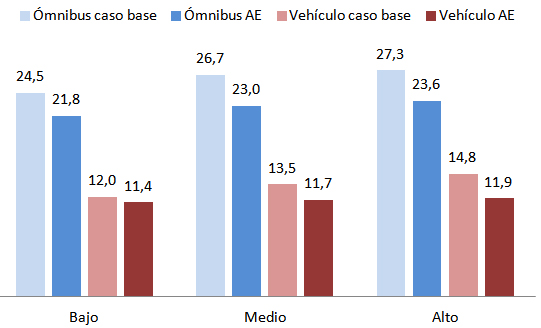
\includegraphics[width=0.8\linewidth]{Figures/duracion_viajes}
	\caption[Comparación de la duración de los viajes en el escenario base y al aplicar el AE.]{Comparación de la duración de los viajes (ómnibus y otros vehículos, en minutos) en el recorrido completo del Corredor Garzón para los diferentes tipos de tráfico.
}
	\label{fig:duracion_viajes}
\end{figure}


\subsection{Valores numéricos al aplicar los cambios (escenario alternativo)}

Para determinar cuales son los cambios que logran mejores rendimientos se elabora la Tabla \ref{table:resultado_alternativo}. Esta tabla se basa en el tráfico medio, ya que sólo se quiere realizar una comparación sencilla de las mejoras realizadas dado que luego se realizaran las evaluaciones aplicando todas las modificaciones para cada uno de los tipos de tráfico estudiados. Las modificaciones presentadas se aplican en el orden que aparece en la tabla y sus valores son acumulativos. Se puede apreciar que la modificación que logra una mayor diferencia es la utilización de paradas alternadas.


\begin{table}[H]
	\renewcommand{\arraystretch}{1.2}
	\caption[Valores numéricos del escenario alternativo]{Valores numéricos del escenario alternativo con su velocidad promedio ómnibus (vpb) y velocidad promedio vehículos(vpv) comparando el \emph{fitness} para el tráfico medio }
	\label{table:resultado_alternativo}
	\centering
	\begin{tabular}{lrrrr }
		\hline
		\textit{modificación del escenario}&
		$vbp(km/h)$& 
		$vvp(km/h)$ & 
		\emph{fitness} &
		mejora(\%)
		\\ 
		\hline
		caso base & 14.59  & 28.81& 12.05 & -\\
		eliminar paradas & 15.44  & 29.03& 12.35 & 2.4\\
		eliminar peatonales  & 16.02  & 29.32& 12.59 & 4.4\\
		paradas alternadas  & 19.17  & 28.88& 13.34 & 10.7\\	
		cambiar reglas de semáforos  & 18.50  & 29.70& 13.39 & 11.1\\				
		\hline
	\end{tabular}
\end{table}

Una vez que se aplican todos las modificaciones sobre el escenario, se realiza un análisis para los demás tipos de tráfico. Como se reporta en la Tabla \ref{table:mejoras_trafico_alternativo}, se obtienen mejores rendimientos en todos los tipos de tráfico estudiados y el mejor rendimiento se obtiene cuando el tráfico es alto. 

\begin{table}[H]
	\renewcommand{\arraystretch}{1}
	\renewcommand{\tabcolsep}{12pt}	
	\caption[Mejoras del escenario alternativo.]{Mejoras del escenario alternativo  para las velocidades promedio de los ómnibus \textit{(vpb)} y de otros vehiculos \textit{(vpv)} en el escenario alternativo para distintos tipos de tráficos }
	\label{table:mejoras_trafico_alternativo}
	\centering
	\begin{tabular}{lrrrr }
		\toprule
		\textit{escenario}&
		$vbp(km/h)$& 
		$vvp(km/h)$ & 
		\textit{fitness} &
		\textit{mejora } \newline \textit{fitness}(\%)
		\\ 
		\midrule
		tráfico bajo & 20.72  & 33.18 & 14.97 & 11.5\\
		tráfico medio & 18.50  & 29.70& 13.39 & 11.1 \\
		tráfico alto  & 18.60  & 27.17& 12.70 & 12.4\\		
		\bottomrule
	\end{tabular}
\end{table}


Luego de obtener los valores para el escenario alternativo se procede a aplicar el AE, cuyos resultados se presentan a continuación.


\subsection{Resultados de la evaluación sobre el escenario alternativo}

El escenario alternativo supuso una mejora sustancial en comparación con el caso base (11 \% en el valor de \emph{fitness}). Se procedió a aplicar el AE para determinar si aún hay posibilidad de mejorar los valores de velocidad y \emph{fitness}.

Los resultados obtenidos se reportan en la Tabla \ref{table:mejoras_trafico_alternativo_algoritmo} y permiten concluir que se mejora claramente el rendimiento del escenario alternativo y por supuesto del caso base en todos los tipos de tráfico. Comparando con la realidad actual, se logran mejoras de hasta 37\% en el valor de \emph{fitness}. 

%Al comparar los resultados obtenidos se aprecia que cuanto mayor es la densidad de tráfico, mayor es el porcentaje de mejora. Además, un resultado interesante es que las diferencias entre los valores de los distintos tipos de tráfico se redujo.

\begin{table}[h]
	\renewcommand{\arraystretch}{1.2}
	\caption[Valores numéricos al aplicar el AE sobre el escenario alternativo.]{Mejoras obtenidas al aplicar el algoritmo evolutivo sobre el escenario alternativo, comparando las velocidades de ómnibus \textit{(vpb)}, otros vehículos \textit{(vpv)} y el \emph{fitness} con cada tipo de tráfico contra el escenario base.}
	\label{table:mejoras_trafico_alternativo_algoritmo}
	\centering
	\begin{tabular}{lrrrrrrr}
		\hline 
		\textit{instancia}& 
		$vbp(km/h)$& 
		$vpv(km/h)$&
		\multicolumn{2}{c}{\emph{fitness}}&  & 
		\multicolumn{2}{c}{mejora \emph{fitness} (\%)}\\  \cline{4-5} \cline{7-8}&     &     & \multicolumn{1}{c}{promedio$\pm\sigma$} & \multicolumn{1}{c}{mejor} &  & \multicolumn{1}{c}{promedio} & \multicolumn{1}{c}{mejor} \\ \hline

	\textit{tráfico bajo} & 23.15$\pm$0.36 & 34.43$\pm$0.33 & 15.99$\pm$0.08 & 16.10 & & 19.1& 19.9 \\
		\textit{tráfico medio} & 21.83$\pm$0.50  & 33.89$\pm$0.22 & 15.47$\pm$0.09& 15.65 & & 28.3 & 29.8\\
		\textit{tráfico alto} & 21.46$\pm$0.54  & 33.41$\pm$0.38 & 15.24$\pm$0.19& 15.50 & & 34.8 & 37.1\\	
		\hline		    
	\end{tabular}
\end{table}

En la gráfica de la Figura \ref{fig:duracion_viajes_alernativo} se comparan las duraciones de los viajes al aplicar el AE sobre el escenario alternativo. Se produce una gran reducción en la duración de los viajes de los ómnibus en los tres tipos de tráfico, mientras para el caso de los vehículos la mayor diferencia ocurre cuando el tráfico es alto.

\begin{figure}[ht]
	\centering
	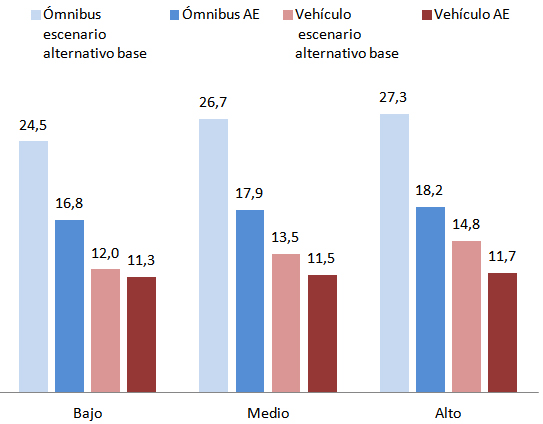
\includegraphics[width=0.8\linewidth]{Figures/duracio_viajes_alternativo}
	\caption[Comparación de la duración de los viajes en minutos entre el escenario base y el algoritmo evolutivo sobre el escenario alternativo.]{Comparación de la duración en minutos de los viajes realizados sobre el escenario base y al aplicar el algoritmo evolutivo  al escenario alternativo, de ómnibus y otros vehículos en el recorrido completo del corredor Garzón, para los diferentes tipos de tráfico.}
	\label{fig:duracion_viajes_alernativo}
\end{figure}

Al aplicar el criterio de significancia estadística para comprobar que la mejora es significativa tanto al comparar con los valores del caso base como con los del escenario alternativo se determina que efectivamente existe evidencia estadística que soporta esta hipótesis.

\subsection{Variación de la función de \emph{fitness}}

La función de \emph{fitness} propuesta (Ecuación \ref{eq:funcion_fitness}) utiliza los pesos \emph{$w_1$ = $w_2$ = 1}, lo que representa un balance equitativo para ómnibus y vehículos. Estos pesos pueden ser modificados en función de lo que se necesite de acuerdo a la realidad de la zona estudiada, por lo que se realizaron experimentos con dos configuraciones de pesos para comparar como varían las velocidades cuando se da más prioridad a un tipo de vehículo sobre el otro.

%Por un cruce de Garzón pasan cada hora:
%70 ómnibus , si aproximamos con 23 personas= 1610 personas por hora
%800 autos, si aproximamos  2 personas por vehículo nos da 1600 personas por hora.
%Una cantidad similar  pasan por el cruce en ambos medios de transporte por lo que no existe una tendencia a favor de una sobre la otra, se podría aproximar que 50\% eligen el ómnibus y 50\% el auto.


\subsubsection{Prioridad para los ómnibus}
Este caso dá más prioridad a los ómnibus, y se justifica por el hecho que uno de los objetivos buscados por la IMM es que se utilice más el transporte colectivo como parte de su Plan de Movilidad Urbana. La premisa es que al mejorar la duración del viaje en ómnibus en relación al viaje en auto por el corredor, las personas optarán por el transporte colectivo. Se experimentó cambiando los pesos de la función de \emph{fitness} con un peso de 70\% para los ómnibus y 30\% al resto de los vehículos.


\subsubsection{Prioridad a otros vehículos}

Este caso asigna 70\% del peso a los vehículos y 30\% a los ómnibus. Es el caso opuesto al anterior y resulta útil para comparar sus resultados. No resulta especialmente relevante en el caso de Garzón, ya que la velocidad promedio de los ómnibus es inferior a la del resto de los  vehículos en todos los casos de tráfico estudiados, pero podrían existir otros escenarios donde se requiera una velocidad promedio superior para el resto de los vehículos.

\subsubsection{Resultados}

La Tabla \ref{table:analisis_fitness} compara las velocidades promedio de ómnibus y vehículos para las tres configuraciones de pesos evaluadas y por cada tipo de tráfico.  El caso 50-50 es el caso base donde los pesos son iguales, 70-30 es el caso con más prioridad para los ómnibus y el 30-70 más prioridad a los otros vehículos. Se analiza cuanto varían las velocidades de ómnibus \emph{(var. vpb)} y otros vehículos \emph{(var. vpv)} comparando contra el caso 50-50 de cada tipo de tráfico.


\begin{table}[H]
	\renewcommand{\arraystretch}{1.2}
	\caption[Valores obtenidos al modificar los pesos de la función de \emph{fitness}.]{Valores obtenidos al modificar los pesos de la función de \emph{fitness} para ómnibus (pb) y otros vehículos (pv). Se reportan las variaciones en la velocidad promedio de ómnibus (vpb), otros vehículos (vpv) y \emph{fitness}, donde el símbolo positivo (+) y negativo(-) indican la variación porcentual de esos valores. }
	\label{table:analisis_fitness}
	\centering
	\begin{tabular}{p{1.2cm}p{1.2cm}p{1.8cm}p{1.8cm}p{1.8cm}p{1.1cm}p{1.1cm}p{1.2cm} }
		\hline
		\textit{instancia} \newline \textit{tráfico} &
		\textit{pb(\%) pv (\%)}& 
		\textit{vpb(km/h)} & 
		\textit{vpv(km/h)} &
		\textit{fitness} &
		\textit{var. \newline vpb(\%)} &
		\textit{var. \newline vpv(\%)} &
		\textit{var.} \newline \emph{fitnesss}(\%)
		\\ 
		\hline
		& 50-50  & 17.92$\pm$0.18 & 34.30$\pm$0.40 & 14.50$\pm$0.14  &- & - & -\\		
		\textit{bajo} & 70-30  & 17.93$\pm$0.23 & 34.06$\pm$0.17 & 12.65$\pm$0.11  & +0.07 & -0.70 & -12.79\\		
		& 30-70 & 17.55$\pm$0.23 & 34.71$\pm$0.21 & 16.42$\pm$0.10  & -2.06 & +1.18 & +13.21\\
		\hline
		
		& 50-50  & 16.95$\pm$0.32 & 33.29$\pm$0.29 & 13.95$\pm$0.15  &- & - & -\\		
		\textit{medio} & 70-30  & 17.29$\pm$0.27 & 33.08$\pm$0.14 & 12.24$\pm$0.12  & +2.0 & -0.62 & -12.30\\		
		& 30-70 & 16.71$\pm$0.42 & 33.79$\pm$0.31 & 15.92$\pm$0.11  & -1.41 & +1.49& +14.11\\
		
		\hline
		& 50-50  & 16.51$\pm$0.60 & 32.90$\pm$0.25 & 13.72$\pm$0.17  &- & - & -\\		
		\textit{alto} & 70-30  & 16.72$\pm$0.14 & 32.79$\pm$0.26 & 13.75$\pm$0.07  & +1.24 & -0.33 & +0.19\\	
		& 30-70 & 15.48$\pm$0.42 & 33.20$\pm$0.25 & 15.49$\pm$0.16  & -6.23 & +0.92 & +12.87\\
		\hline
	\end{tabular}
\end{table}


Los resultados indican que al variar los pesos de la función de \emph{fitness} las velocidades promedio de los vehículos se ven afectadas. Al dar más prioridad a los ómnibus se produce, como cabía esperar, un aumento en su velocidad promedio y una leve baja en la velocidad promedio del resto de los vehículos. Cuando el tráfico es bajo este cambio casi no aumenta la velocidad de los ómnibus. Una explicación posible de este comportamiento es que ya se llegó a un limite máximo de velocidad de circulación y no se puede mejorar por sobre ese valor.

Al dar más prioridad a los otros vehículos se produce un aumento en su velocidad y una disminución en la velocidad de los ómnibus, la cual es muy evidente en el caso de tráfico alto. Este resultado permite apreciar como estos valores son fuertemente afectados por la densidad de tráfico que se estudie.

En general las variaciones en las velocidades no son grandes, pero son lo suficientemente apreciables para tener cierta flexibilidad al plantear distintos objetivos que tiendan a favorecer un tipo u otro de vehículos en diferentes situaciones de tráfico.


\subsection{Eficiencia computacional}

Se llevó a cabo un estudio de la eficiencia computacional del AE implementado, para analizar los tiempos de ejecución cuando se usan varios procesadores y cómo se desempeña su capacidad de paralelismo.

Para estudiar la eficiencia en diferentes contextos, se evalúan nueve ejecuciones del AE; tres con cada tipo de tráfico considerado: alto, medio y bajo, para estudiarlo en diferentes contextos. El algoritmo utiliza 32 hilos de ejecución para realizar las simulaciones de tráfico,	 por lo que se emplea esa cantidad de núcleos.

Las pruebas fueron realizadas sobre el equipo node40 del Cluster FING, con un procesador AMD Opteron 6272 2.09GHz, 48 GB RAM y 32 núcleos utilizados.

Para evaluar la eficiencia se calcula el \emph{speedup}. El \emph{speedup} (${S_N}$) es una métrica que evalúa la mejora de rendimiento de una aplicación paralela al aumentar la cantidad de procesadores, comparando con el rendimiento al usar un solo procesador (Ecuación \ref{eq:funcion_speedup}). En la definición de ${S_N}$, ${T_1}$ es el tiempo de ejecución del algoritmo serial o secuencial, y ${T_N}$ el tiempo del algoritmo ejecutado sobre N procesadores. El resultado ideal es obtener \emph{speedup} lineal (${S_N}$ = N), pero en la práctica utilizar N procesadores no garantiza una mejora de factor N; lo habitual es obtener un \emph{speedup} menor al ideal o \emph{speedup} sublineal, posibles causas para este comportamiento son: que el procesamiento no sea del todo paralelizable, demoras en las comunicaciones y sincronizaciones, tiempos ociosos, etc.

\begin{equation}
\label{eq:funcion_speedup}
{S_N} = \frac{T_1}{T_N}
\end{equation}



La eficiencia computacional (${E_N}$) corresponde al valor normalizado del \emph{speedup} (entre 0 y 1) respecto a la cantidad de procesadores. Los valores cercanos a uno indican una alta eficiencia computacional.
\begin{equation}
\label{eq:funcion_eficiencia}
{E_N} = \frac{T_1}{N*T_N} = \frac{S}{N}
\end{equation}

 La Tabla \ref{table:analisis_speedup} reporta los resultados numéricos del análisis de eficiencia computacional. Los resultados indican que el algoritmo paralelo logra una mejora sustancial en los tiempos de ejecución, con un valor promedio del \emph{speedup} de 25.7 y eficiencia promedio de 0.8 al utilizar 32 recursos de cómputo. Estos valores corresponden a un \emph{speedup} sublineal, pero pueden considerarse como buenos valores de las métricas de eficiencia computacional.

\begin{table}[H]
	\renewcommand{\arraystretch}{1.2}
	\caption[Análisis de la eficiencia computacional.]{Análisis de la eficiencia computacional comparando los tiempos de ejecución secuencial y paralela (en minutos). Se presentan las nueve ejecuciones realizadas, tres por cada tipo de tráfico. }
	\label{table:analisis_speedup}
	\centering
	\begin{tabular}{ccrrrr}
		\hline
		
		\#&
		\emph{tipo de \newline tráfico} &
		\emph{serial (m)} & 
		\emph{paralelo (m)} &
		\emph{speedup} &
		\emph{eficiencia}
		\\ 
		\hline
		1& bajo  & 1572 & 59 & 26.64 & 0.83\\
		2& bajo  & 1571 & 59 & 26.62 & 0.83\\
		3& bajo  & 1183 & 44 & \textbf{26.88} & \textbf{0.84}\\
		
		4& medio  & 3002 & 119 & 25.22 & 0.78\\
		5& medio  & 2195 & 82 & 26.76 & 0.83\\
		6& medio  & 3007 & 120 & 25.05 & 0.78\\
		
		7& alto  & 2920 & 110 & 26.5 & 0.82\\
		8& alto  & 4365 & 183 & 23.85 & 0.74\\
		9& alto  & 4276 & 177 & 24.15 & 0.75\\
		\hline
		 &  &  & promedio & 25.7$\pm$1.1 & 0.80$\pm$0.03\\
		
		\hline
	\end{tabular}
\end{table}



La gráfica de la Figura \ref{fig:speedup1} muestra como al aumentar el tráfico de datos disminuye el \emph{speedup}. Este fenómeno sucede porque el \emph{speedup} está influenciado por los accesos al disco duro: al tener más vehículos circulando en la simulación de tráfico requiere leer y escribir más información en los archivos, lo que aumenta el tiempo de ejecución del algoritmo. El impacto del aumento del tráfico sobre el \emph{speedup}, como se puede apreciar en los resultados reportados en la gráfica de la Figura \ref{fig:speedup1}, no es significativo.

\begin{figure}[ht]
	\centering
	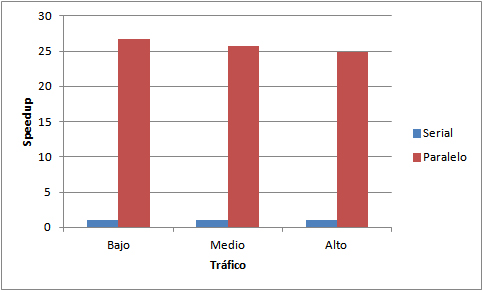
\includegraphics[width=0.8\linewidth]{Figures/speedup1}
	\caption[Comparación de los \emph{speedup} promedios para cada tipo de tráfico.]{Comparación de los \emph{speedup} promedios para cada tipo de tráfico. Se representa el caso serial que corresponde al \emph{speedup} = 1 para fines de comparación.}
	\label{fig:speedup1}
\end{figure}
